% Regenerate with latex and dvisvgm; see graph-matching-common.tex.
% Shared styles for the vector replacements in graph-matching/.
% Compile each diagram from this directory, for example:
% latex -interaction=nonstopmode -halt-on-error augment-1.tex
% dvisvgm --no-fonts --exact --bbox=papersize -o augment-1.svg augment-1.dvi
\documentclass[tikz,border=5pt]{standalone}
\usepackage{lmodern,amssymb}
\usetikzlibrary{arrows.meta,backgrounds,calc}
\definecolor{matchred}{HTML}{D7191C}
\definecolor{matchblue}{HTML}{1748B5}
\definecolor{blossomgreen}{HTML}{087A16}
\definecolor{blossomfill}{HTML}{B3E3AF}
\tikzset{
  diagram/.style={x=1mm,y=-1mm,font=\small,line width=.6pt,
    line cap=round,line join=round,
    background rectangle/.style={fill=white},show background rectangle},
  vertex/.style={circle,draw,fill=white,minimum size=5mm,inner sep=0pt},
  point/.style={circle,fill=black,minimum size=2.8mm,inner sep=0pt},
  exposed/.style={point,draw=matchred,fill=matchred!80,line width=1pt},
  matching/.style={line width=2pt},
  transition/.style={-{Stealth[length=4mm,width=3mm]},
    line width=1.4pt,draw=matchblue},
  blossom/.style={draw=blossomgreen,fill=blossomfill,line width=1pt},
  route/.style={draw=matchred,line width=.9pt},
  label/.style={inner sep=1.5pt,align=center},
}

% The five-cycle has exactly two matching edges. Its exposed base is b0.
% Call inside a scope to translate the entire blossom consistently.
\newcommand{\FiveBlossom}{%
  \draw[blossom] (16,0) circle[radius=22mm];
  \foreach \id/\px/\py in {b0/0/0,b1/12/-16,b2/29/-9,b3/29/10,b4/11/16}
    \node[point] (\id) at (\px,\py) {};
  \draw (b0) -- (b1) (b2) -- (b3) (b4) -- (b0);
  \draw[matching] (b1) -- (b2) (b3) -- (b4);
  \node[label,text=blossomgreen,above] at (16,-22) {blossom};
  \node[label,text=blossomgreen,above=.3mm,xshift=-2mm] at (b0.north) {root};
  \node[label,below=.5mm] at (b0.south) {$v$};
}

\begin{document}
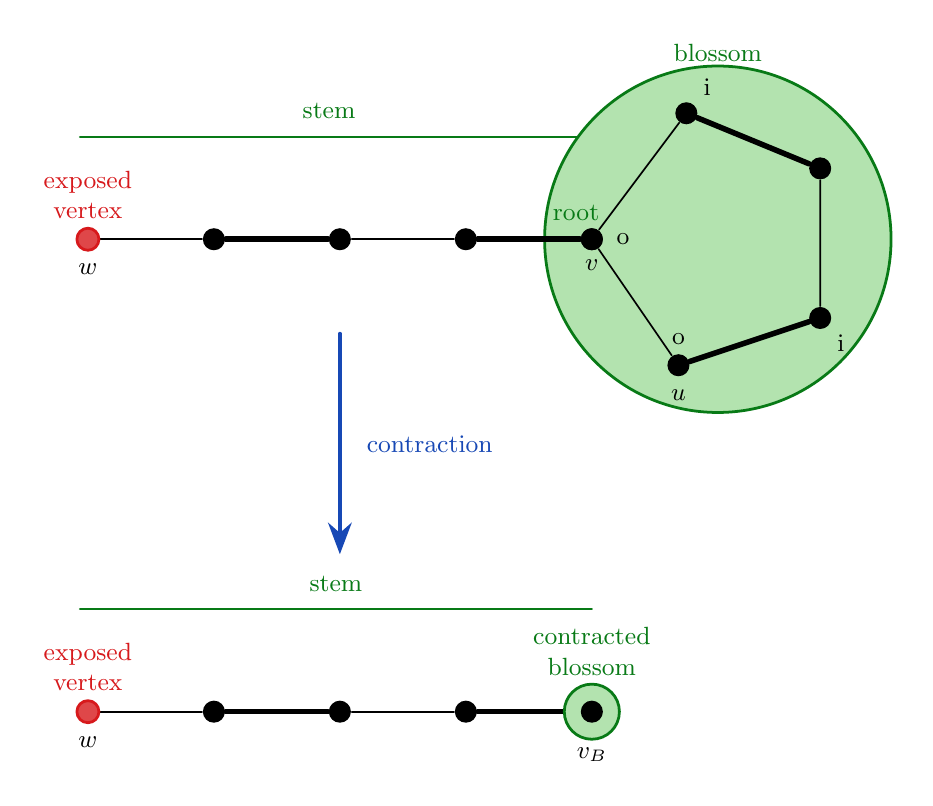
\begin{tikzpicture}[diagram]
  \begin{scope}[xshift=64mm,yshift=0mm]
    \FiveBlossom
    \node[label,above right=.5mm] at (b1.north east) {$\mathrm{i}$};
    \node[label,below right=.5mm] at (b3.south east) {$\mathrm{i}$};
    \node[label,above=.5mm] at (b4.north) {$\mathrm{o}$};
    \node[label,below=1mm] at (b4.south) {$u$};
    \node[label,right=1mm] at (b0.east) {$\mathrm{o}$};
  \end{scope}
  \foreach \row in {0,60} {
    \begin{scope}[shift={(0,\row)}]
      \foreach \i in {0,1,2,3,4}
        \node[point] (s\row-\i) at (16*\i,0) {};
      \draw (s\row-0) -- (s\row-1) (s\row-2) -- (s\row-3);
      \draw[matching] (s\row-1) -- (s\row-2) (s\row-3) -- (s\row-4);
      \node[exposed] at (s\row-0) {};
      \node[label,text=matchred,above=2mm] at (s\row-0) {exposed\\vertex};
      \node[label,below=1mm] at (s\row-0.south) {$w$};
      \ifnum\row=0 \def\stemend{62.25}\else \def\stemend{64}\fi
      \draw[blossomgreen,line width=.8pt] (-1,-13) -- (\stemend,-13)
        node[midway,above=1mm] {stem};
    \end{scope}
  }
  \draw[blossom] (64,60) circle[radius=3.5mm];
  \node[point] at (64,60) {};
  \node[label,text=blossomgreen,above=4mm] at (64,60) {contracted\\blossom};
  \node[label,below=4mm] at (64,60) {$v_B$};
  \draw[transition] (32,12) -- (32,40)
    node[midway,right=2mm,text=matchblue] {contraction};
\end{tikzpicture}
\end{document}
